% tbkit: a verified toolkit for tight-binding models
%
% Draft for SciPost Physics Codebases. Written with the standard article
% class: move the body into SciPost's template (SciPost.cls) before
% submission. Figures and tables come from paper/figures/build_all.py.
\documentclass[11pt,a4paper]{article}

\usepackage[margin=2.5cm]{geometry}
\usepackage{amsmath,amssymb}
\usepackage{graphicx}
\usepackage{booktabs}
\usepackage{tabularx}
\usepackage{siunitx}
\usepackage{xcolor}
\usepackage{listings}
\usepackage{hyperref}
\usepackage{tikz}
\usetikzlibrary{arrows.meta,positioning}

\lstset{language=Python, basicstyle=\ttfamily\footnotesize, columns=fullflexible,
        keywordstyle=\color{blue!60!black}, commentstyle=\color{gray}, frame=lines,
        breaklines=true, showstringspaces=false}
\newcommand{\code}[1]{\texttt{#1}}
% table rows from paper/figures/build_all.py (the primitive \input is safe inside tabular)
\makeatletter\newcommand{\rows}[1]{\@@input #1.tex }\makeatother
\graphicspath{{figures/}}
\newcommand{\tbkitversion}{0.4.2}
\newcommand{\kwantversion}{1.5.0}
\newcommand{\pythtbversion}{2.0.2}
\newcommand{\numpyversion}{2.5.3}
\newcommand{\scipyversion}{1.18.1}

\IfFileExists{tables/bench_setup.tex}{\newcommand{\benchnorb}{32}
\newcommand{\benchnk}{200}
\newcommand{\benchplatform}{macOS-26.6.2-arm64-arm-64bit}
}{}

\title{tbkit: a verified Python toolkit for tight-binding models,\\
       from band topology to quantum transport}
\author{Charles Poli\thanks{\href{mailto:cpoli374@gmail.com}{cpoli374@gmail.com}}}
\date{Codebase release \tbkitversion}

\begin{document}
\maketitle

\begin{abstract}
tbkit is an open-source Python package that builds and solves tight-binding
models in one, two and three dimensions, written in vectorized NumPy and
SciPy. One model definition serves finite lattices and Bloch Hamiltonians.
On these models tbkit computes band structures and densities of states;
topological invariants (Chern, spin and mirror Chern, $\mathbb{Z}_2$, Bott,
higher-order, Majorana); Kubo response (Hall, Nernst, thermal Hall,
orbital magnetization, linear and nonlinear optics); and quantum transport
from the scattering matrix of exact lead modes. It also covers Floquet
drives, non-Hermitian bands with exceptional points, moir\'e supercells,
Wannier functions, and Hubbard and Bogoliubov--de Gennes mean field.
The package is built around verification. Every argument is validated,
the 746 unit tests cover every line, and each of the 85 gallery examples
asserts its key numbers before plotting, so the documentation states
nothing that the code does not check on every commit. We describe the
design and the algorithms, present a worked example from bands to
transport, and validate tbkit against Kwant~\cite{groth2014} and
PythTB~\cite{pythtb}. The two independent packages agree with tbkit to
within $10^{-12}$ on transmissions, lead modes, Berry phases and Wannier
centres. We also benchmark tbkit against both and state where each one is
the better choice.
\end{abstract}

\tableofcontents

%----------------------------------------------------------------------------
\section{Introduction}
\label{sec:intro}

Tight-binding models are among the most widely used tools of condensed-matter physics. They
describe the bands of graphene and of transition-metal dichalcogenides,
quantum Hall and topological insulators, disordered conductors and
mesoscopic devices, and they are the reference language for teaching band
theory. Several mature packages serve parts of this landscape.
Kwant~\cite{groth2014} computes quantum transport through large devices.
PythTB~\cite{pythtb} and Z2Pack~\cite{gresch2017} focus on Berry phases and
topological invariants, and TBmodels~\cite{gresch2018} and
WannierTools~\cite{wu2018} work with Wannier90~\cite{pizzi2020}
Hamiltonians of real materials. pybinding~\cite{pybinding} targets large
real-space systems with the kernel polynomial method.

A typical project, however, crosses these boundaries. A researcher studying
a Chern insulator wants its bands, its Chern number, its Hall conductivity
at arbitrary filling, the edge states of a ribbon, and the conductance of
a device cut from the same model, possibly with disorder or a periodic
drive. With separate packages, the model has to be rewritten for each, in
different conventions for the Bloch gauge, the hopping direction or the
sign of the Hall conductivity. Each rewrite can introduce errors.

tbkit addresses this with a single model definition and a broad
set of tools that act on it (Sec.~\ref{sec:design}). We do not claim it is
the fastest package for any one task: Kwant scales further for large
transport calculations, and PythTB~2 is now as fast as tbkit on Bloch
meshes (Sec.~\ref{sec:performance}). What tbkit provides is breadth in
one package, with mechanics that a user can inspect, and verification
throughout. Every numerical claim in its documentation is asserted by code that
runs in continuous integration (CI), and its results agree with Kwant and
PythTB to near machine precision (Sec.~\ref{sec:validation}).

This paper is organized as a user guide. Section~\ref{sec:design} describes the design.
Sections~\ref{sec:building} to~\ref{sec:beyond} cover the physics, and
Sec.~\ref{sec:example} works through one complete example.
Section~\ref{sec:validation} validates the results and
Sec.~\ref{sec:performance} measures performance. Section~\ref{sec:teaching}
describes the gallery as teaching material.

%----------------------------------------------------------------------------
\section{Design}
\label{sec:design}

\begin{figure}[t]
\centering
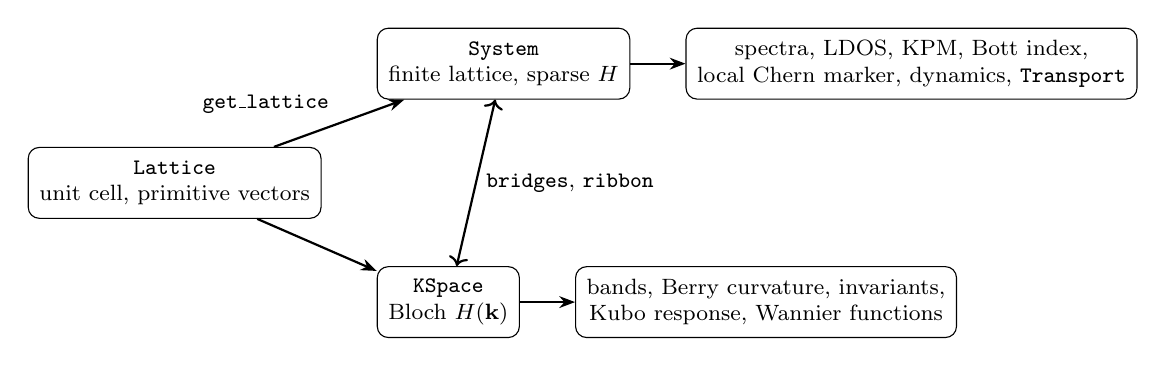
\begin{tikzpicture}[node distance=6mm and 7mm, every node/.style={font=\footnotesize},
  box/.style={draw, rounded corners, align=center, minimum height=9mm, inner sep=4pt},
  arr/.style={-{Stealth[length=2mm]}, thick}]
\node[box] (lat) {\code{Lattice}\\ unit cell, primitive vectors};
\node[box, above right=of lat] (sys) {\code{System}\\ finite lattice, sparse $H$};
\node[box, below right=of lat] (ks) {\code{KSpace}\\ Bloch $H(\mathbf{k})$};
\node[box, right=of sys] (rs) {spectra, LDOS, KPM, Bott index,\\ local Chern marker, dynamics, \code{Transport}};
\node[box, right=of ks] (kk) {bands, Berry curvature, invariants,\\ Kubo response, Wannier functions};
\draw[arr] (lat) -- node[above left] {\code{get\_lattice}} (sys);
\draw[arr] (lat) -- (ks);
\draw[arr, <->] (sys) -- node[right, align=left] {\code{bridges}, \code{ribbon}} (ks);
\draw[arr] (sys) -- (rs);
\draw[arr] (ks) -- (kk);
\end{tikzpicture}
\caption{The two pipelines of tbkit. Both start from a \code{Lattice}; the
\code{bridges} module converts a Bloch model into a finite \code{System} and
back, and \code{ribbon} cuts a periodic model into a ribbon or slab, which
also serves as a transport lead.}
\label{fig:design}
\end{figure}

\paragraph{Two pipelines.} A \code{Lattice} holds a unit cell (orbital
positions and one-character sublattice tags) and primitive vectors
(Fig.~\ref{fig:design}). In real space, \code{get\_lattice} repeats the cell, geometry methods
cut flakes, discs or ribbons, and a \code{System} sets hoppings by neighbour
order, angle or sublattice pair. Modifiers then act on the stored
hoppings: disorder, defects, strain, and Peierls phases for magnetic fields.
\code{get\_ham} assembles a sparse matrix. In reciprocal space, a
\code{KSpace} takes hoppings as an orbital pair and a lattice offset
$\mathbf{R}$ and returns $H(\mathbf{k})$. Every specialized model returns a
\code{KSpace}, so every band and topology tool applies to it. These include
magnetic supercells, Slater--Koster multi-orbital models~\cite{slater1954},
Bogoliubov--de Gennes Hamiltonians, Floquet Hamiltonians, moir\'e
supercells, discretized $k\cdot p$ models and Wannier90 imports.

\paragraph{One Bloch sum, one eigensolver.} Every Bloch matrix in the package
comes from one vectorized routine (\code{KSpace.\_bloch\_sum}). This holds
for the Hamiltonian, overlaps, velocities $\partial_\mu H$, vector-potential
couplings and Floquet grids. The routine evaluates many $\mathbf{k}$ at once,
with optional analytic derivatives. Every diagonalization over a mesh
goes through one stacked eigensolver (\code{KSpace.\_eigs}), in
memory-bounded chunks and optionally across threads. Optimizing or
correcting these two routines therefore affects every method built on
them.

\paragraph{Conventions.} $H(\mathbf{k})$ uses the periodic gauge (orbital
positions ignored), which leaves eigenvalues and integrated invariants
unchanged. Wilson loops, Wannier centres and the quantum metric add
the positions back when requested (\code{positions=True}), which is the
convention of PythTB. The Hall conductivity follows the TKNN sign, so in a gap
it equals the Chern number returned by \code{chern\_number}. The
conventions are stated in the docstrings and pinned by tests.

\paragraph{Value functions.} Hoppings and onsite energies may be functions
of the sites and of named parameters, \code{t(site\_i, site\_j, **params)}.
\code{get\_ham(**params)} evaluates them, so a parameter sweep or a phase
diagram reuses one model, as with Kwant's value functions.

\paragraph{Validation.} Each public method first validates its arguments
through one module (\code{error\_handling}, 251 checks), which raises an
explicit error naming the problem, for example
the missing lead orbitals of an incomplete interface cell, or a band group of
a non-Hermitian model without a line gap.

\paragraph{Verification policy.} The test suite runs on Python 3.10--3.14,
plus a job on the oldest NumPy, SciPy and matplotlib the package declares.
It covers every line, and any warning fails it. A fixed bug gets a test
that pins it. The 85 gallery examples are executed by every documentation
build, which CI runs on each push, and each asserts its key numbers before
plotting. A change that breaks the physics of an example therefore fails
CI. Section~\ref{sec:validation} adds independent checks against Kwant and
PythTB.

%----------------------------------------------------------------------------
\section{Building models}
\label{sec:building}

\begin{figure}[t]
\centering
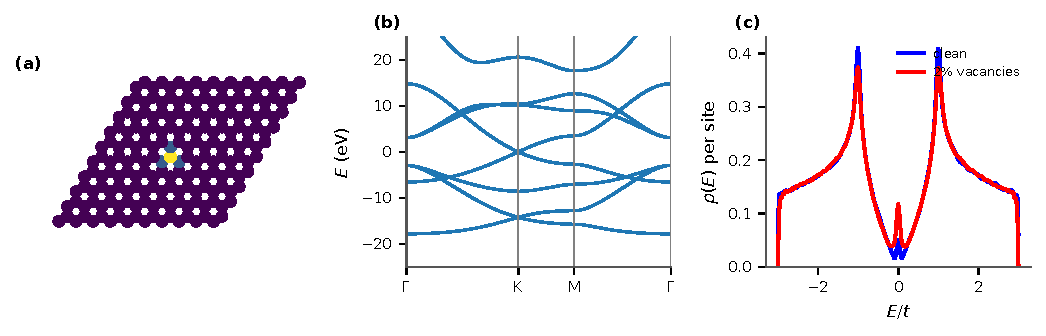
\includegraphics[width=\textwidth]{fig_models}
\caption{Building and solving models.
(a)~An impurity binds a state below the band of a graphene flake.
(b)~Slater--Koster $sp^3$ bands of graphene, with overlaps (a generalized
eigenproblem). (c)~Kernel-polynomial density of states of a 45\,000-site
lattice, clean and with 2\% vacancies.}
\label{fig:models}
\end{figure}

\paragraph{Lattices and geometry.} Ready-made lattices (chain, square,
triangular, honeycomb, kagome, Lieb) and arbitrary unit cells in 1D, 2D
and 3D are supported. Geometry operations remove sites, cut by lines or
ellipses, rotate, and close the boundaries into a torus or cylinder. On a
torus, every bond vector uses the minimum-image convention. Neighbour
search switches from dense distances to a $k$-d tree above 5000 sites.

\paragraph{Several orbitals and spin.} \code{OrbitalSystem} attaches
orbitals ($s$, $p$, $d$) and spin to each site, and builds hopping blocks
from Slater--Koster parameters, intrinsic and Rashba spin--orbit coupling,
or explicit matrices [Fig.~\ref{fig:models}(b)]. Overlaps turn every
eigenproblem into a generalized one.

\paragraph{From continuum to lattice.} \code{discretize} turns a $k\cdot p$
Hamiltonian, written in SymPy, into a lattice model on a chain, square or
cubic grid. Its parameters can stay symbolic and become value functions.

\paragraph{Wannier functions.} \code{read\_wannier90} imports
\code{\_hr.dat} models. \code{wannierize} builds maximally localized Wannier
functions of any \code{KSpace} model~\cite{marzari1997}, with
Souza--Marzari--Vanderbilt disentanglement for entangled bands~\cite{souza2001}. Its result
interpolates the bands through a Wannier-basis \code{KSpace}.

\paragraph{Large systems.} Sparse shift-invert diagonalization, the kernel
polynomial method~\cite{weisse2006} [Fig.~\ref{fig:models}(c)], and a
recursive Green's function for long quasi-one-dimensional devices
extend real-space calculations to $10^5$ sites and more.

%----------------------------------------------------------------------------
\section{Band topology}
\label{sec:topology}

\begin{figure}[t]
\centering
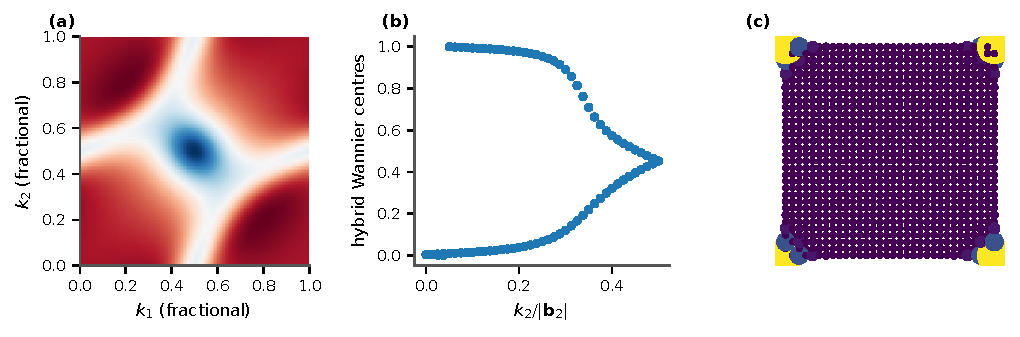
\includegraphics[width=\textwidth]{fig_topology}
\caption{Band topology. (a)~Berry curvature of the lower band of the
Haldane model over the Brillouin zone. (b)~Wilson-loop (hybrid Wannier
centre) flow of the occupied pair of the Kane--Mele model: the centres
wind, so $\mathbb{Z}_2 = 1$. (c)~Corner states of a finite quadrupole
insulator.}
\label{fig:topology}
\end{figure}

Chern numbers use the gauge-invariant plaquette method of Fukui, Hatsugai and
Suzuki~\cite{fukui2005}. On a coarse mesh it gives an integer
whenever the gap stays open [Fig.~\ref{fig:topology}(a)]. Spin and mirror
Chern numbers project onto the eigenspaces of $s_z$ or of a mirror operator
first. Wilson loops give Berry and Zak phases, hybrid Wannier centres and
their flow~\cite{soluyanov2011}, from which the $\mathbb{Z}_2$ invariant
is read in 2D [Fig.~\ref{fig:topology}(b)] and the four 3D indices
follow. Inversion-symmetric models also give Fu--Kane
parities~\cite{fu2007}. In real space, tbkit computes the local Chern
marker~\cite{bianco2011}, the Bott index~\cite{loring2010} and the
entanglement spectrum, so disordered or finite samples need no
translation symmetry. Nested Wilson loops and corner charges diagnose
higher-order phases~\cite{benalcazar2017} [Fig.~\ref{fig:topology}(c)].
\code{find\_weyl\_points} locates Weyl nodes and their chiralities from
the flux through small spheres. For superconductors, \code{bdg} gives
Kitaev's Majorana number from the Pfaffian~\cite{kitaev2001}, and the
symmetry tools classify a Hamiltonian in the tenfold way.

%----------------------------------------------------------------------------
\section{Response and transport}
\label{sec:response}

\begin{figure}[t]
\centering
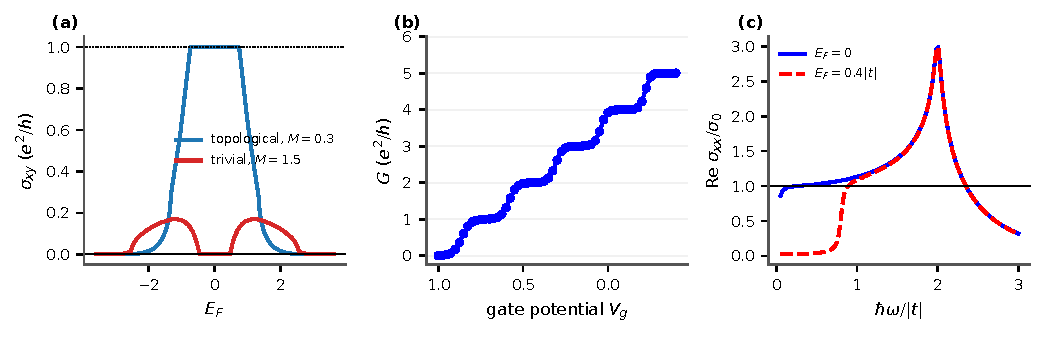
\includegraphics[width=\textwidth]{fig_response}
\caption{Response and transport. (a)~Anomalous Hall conductivity of the
Haldane model against the Fermi level: a plateau at $C=1$ in the gap of the
topological phase, a non-quantized value in the bands. (b)~Conductance
steps of a quantum point contact. (c)~Optical conductivity of graphene,
which approaches the universal value $\sigma_0 = e^2/4\hbar$ at low
frequency.}
\label{fig:response}
\end{figure}

\paragraph{Kubo response.} The anomalous and spin Hall conductivities are
evaluated from the Kubo formula at any Fermi level and temperature, with
analytic velocities $\partial_\mu H$ from the hoppings
[Fig.~\ref{fig:response}(a)]. The orbital magnetization, the anomalous
Nernst and thermal Hall conductivities, and the axion angle share the same
code with different occupation weights. Linear optical conductivity, the
Berry-curvature dipole and the shift current cover optics
[Fig.~\ref{fig:response}(c)]. In real space, the kernel polynomial method
evaluates the Kubo--Bastin formula on large disordered tori.

\paragraph{Scattering matrix.} \code{Transport} holds a sparse device and
its leads. A lead is given as matrices or attached automatically from a
ribbon \code{KSpace}, by matching positions and tags. The lead modes solve
the transfer-matrix pencil with a QZ decomposition. They are normalized to
unit current, and evanescent modes are kept in an ordered Schur basis. The
scattering matrix then follows from one sparse LU factorization of the
device with the lead boundary conditions, as in Kwant~\cite{groth2014}.
Because no broadening $\eta$ enters, results stay exact up to the band
edges of the leads. A conservation law, such as $\sigma_z$ or the
electron--hole $\tau_z$, splits the modes into blocks for spin-resolved
transport or Andreev reflection. Scattering states, their local density of
states, finite temperature and thermoelectric coefficients build on the
same factorization [Fig.~\ref{fig:response}(b)].

\paragraph{Green's functions.} Caroli formulas with Sancho--Rubio
leads~\cite{sancho1985} give multi-terminal conductance matrices, bond
currents and shot noise. \code{surface\_spectral\_function} gives the
spectral function of a semi-infinite crystal, for example the Dirac cone on
the surface of a 3D topological insulator.

%----------------------------------------------------------------------------
\section{Driven, open and interacting systems}
\label{sec:beyond}

\begin{figure}[t]
\centering
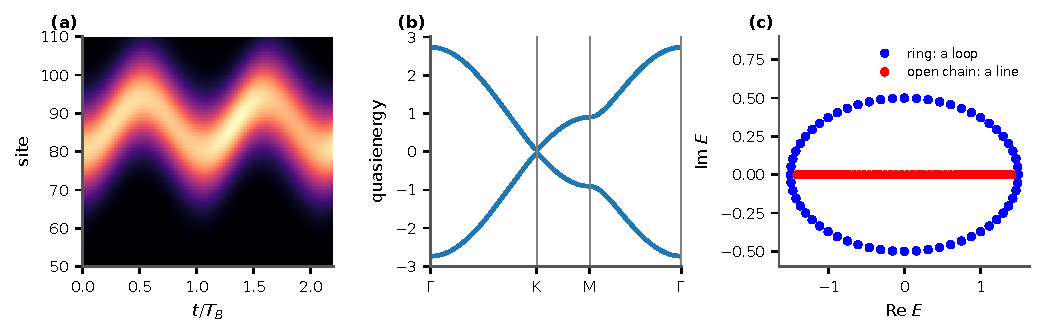
\includegraphics[width=\textwidth]{fig_driven}
\caption{Driven and open systems. (a)~Bloch oscillations of a wavepacket
in a tilted chain. (b)~Floquet bands of graphene under circularly
polarized light, gapped at $K$. (c)~Skin effect in the Hatano--Nelson
chain: the spectrum of a ring winds around a loop, while the open chain
has a real spectrum.}
\label{fig:driven}
\end{figure}

\paragraph{Floquet.} Any $H(\mathbf{k}, t)$ becomes a Floquet
\code{KSpace} whose Hamiltonian is $H_F(\mathbf{k})$, so every band and
topology tool applies to it [Fig.~\ref{fig:driven}(b)]. Step drives are
exact. The winding number of Rudner \emph{et al.}~\cite{rudner2013}
identifies anomalous phases that the Chern numbers of $H_F$ miss.

\paragraph{Non-Hermitian bands.} Non-reciprocal hoppings, gain and loss are
first-class. Biorthogonal Berry curvature and Chern numbers apply to
line-gapped bands, and the spectral winding and generalized Brillouin zone
describe the skin effect [Fig.~\ref{fig:driven}(c)]. The module
\code{exceptional} follows eigenvalues by continuation along a closed loop,
without sorting them. From this it computes vorticities and the band swap
on encircling an exceptional point, and finds exceptional points and their
charges from the discriminant of the characteristic polynomial.

\paragraph{Interactions and dynamics.} Hubbard mean field (collinear and
non-collinear) and the self-consistent Bogoliubov--de Gennes gap equation
work on finite systems. Twisted-bilayer supercells with band unfolding
reach the flat bands at the magic angle~\cite{bistritzer2011}.
Crank--Nicolson propagation follows wavepackets and adiabatic pumping
[Fig.~\ref{fig:driven}(a)].

%----------------------------------------------------------------------------
\section{A worked example: the Haldane model, from bands to transport}
\label{sec:example}

Listing~\ref{lst:haldane} follows one model, Haldane's Chern
insulator~\cite{haldane1988}, through the whole package. The listing is
the file \code{paper/listings/haldane\_workflow.py} of the repository, which
CI runs, so the code printed here is code that passes.

\lstinputlisting[caption={The Haldane model from its bands to its
conductance. Every step asserts its result.}, label=lst:haldane,
firstline=2]{../listings/haldane_workflow.py}

The model is built once (step 1), from graphene's three nearest-neighbour
bonds and the complex second-neighbour hopping $\pm i t_2$. Step 2 checks
the gaps at the two valleys, $2|M \mp 3\sqrt3\,t_2|$. Step 3 computes the
Chern number of the lower band, $C = +1$, and the Hall conductivity with
the Fermi level in the gap, $\sigma_{xy} = C\,e^2/h$, from two independent
algorithms: plaquette fluxes and the Kubo formula. Step 4 cuts a ribbon
from the same hopping list and finds states in the bulk gap. Step 5 turns
the Bloch model into a finite device (\code{finite\_system}), attaches the
ribbon as leads on both sides, and finds the transmission $T = 1$ carried by
the single chiral edge channel. The whole script runs in under a second on
a laptop.

%----------------------------------------------------------------------------
\section{Validation}
\label{sec:validation}

We validate tbkit at three levels.

\paragraph{Against Kwant.} We build three devices independently in tbkit and in
Kwant~\kwantversion, on identical site positions:
a square-lattice strip with a smooth antidot, a disordered graphene device
with zigzag-ribbon leads, and a strip with Rashba spin--orbit coupling and
spin-conserving leads. We compare gauge-invariant quantities: the momenta
and velocities of the lead modes, the transmission, the transmission
eigenvalues (squared singular values of $t$), and the four spin-resolved
blocks of $S$. The comparison covers 37 to 53 energies per device.

\paragraph{Against PythTB.} We build the Haldane and Kane--Mele models with
PythTB~\pythtbversion's own model library and carry them into tbkit
through their hopping lists only. Each package then computes band energies,
Chern numbers, Berry phases, the quantum metric and Berry curvature, and
hybrid Wannier centres on its own. tbkit's $\mathbb{Z}_2$ invariant
reproduces the phase diagram: $\mathbb{Z}_2 = 1$ in the quantum spin Hall
phase and 0 in the trivial phase.

\begin{figure}[t]
\centering
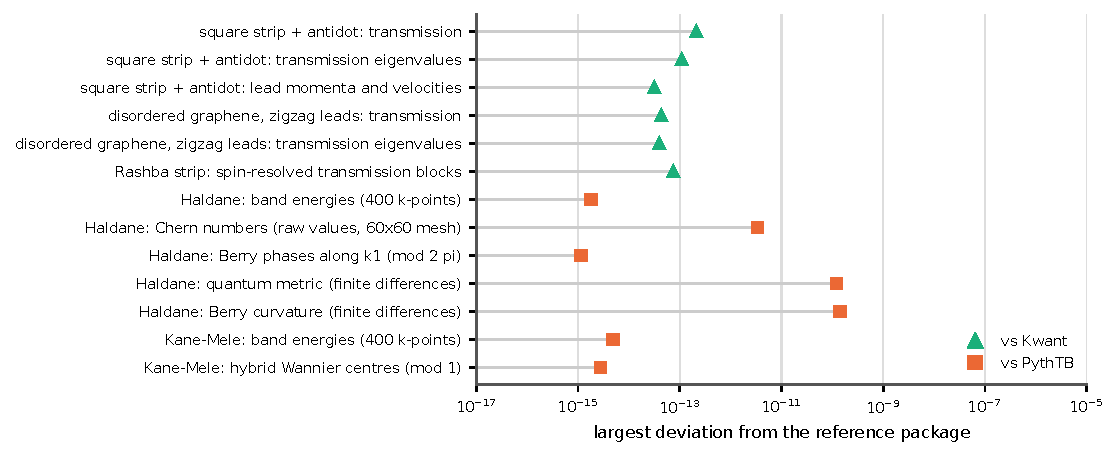
\includegraphics[width=0.8\textwidth]{fig_validation}
\caption{Largest deviation between tbkit and the reference package for
each cross-check (Table~\ref{tab:crosschecks}). The quantum metric and Berry
curvature are finite-difference derivatives in both packages, which limits
their agreement to about $10^{-10}$.}
\label{fig:validation}
\end{figure}

\begin{table}[t]
\centering\small
\caption{Cross-checks of tbkit \tbkitversion{} against Kwant and PythTB (NumPy
\numpyversion, SciPy \scipyversion). Each deviation is the largest absolute
difference over all energies, $k$-points or loops. Each is asserted by
\code{paper/validation/run\_all.py}.}
\label{tab:crosschecks}
\begin{tabular}{llr}
\toprule
Reference & Quantity & Largest deviation \\
\midrule
\rows{tables/crosschecks}
\bottomrule
\end{tabular}
\end{table}

All 13 comparisons agree to within $10^{-12}$, except the two
finite-difference quantities, which agree to $10^{-10}$
(Fig.~\ref{fig:validation}, Table~\ref{tab:crosschecks}).

\paragraph{Against closed-form results.} Table~\ref{tab:analytic} lists
results that gallery examples reproduce and assert. Among them are TKNN
Hall conductances, Zak phases, conductance quantization, graphene's
universal absorption, the BCS gap ratio, Andreev reflection, Majorana
numbers, the anomalous Floquet winding and exceptional-point vorticities.
The validation script re-runs each of these examples.

\begin{table}[t]
\centering\scriptsize
\caption{Closed-form and literature results asserted by the gallery
examples (folder \code{examples/}), with the tolerance of each assert.}
\label{tab:analytic}
\begin{tabularx}{\textwidth}{>{\raggedright\arraybackslash}X>{\raggedright\arraybackslash}p{3.6cm}>{\raggedright\arraybackslash}p{4.2cm}l}
\toprule
Result & Reference & Example & Tolerance \\
\midrule
\rows{tables/analytic}
\bottomrule
\end{tabularx}
\end{table}

%----------------------------------------------------------------------------
\section{Performance}
\label{sec:performance}

\begin{figure}[t]
\centering
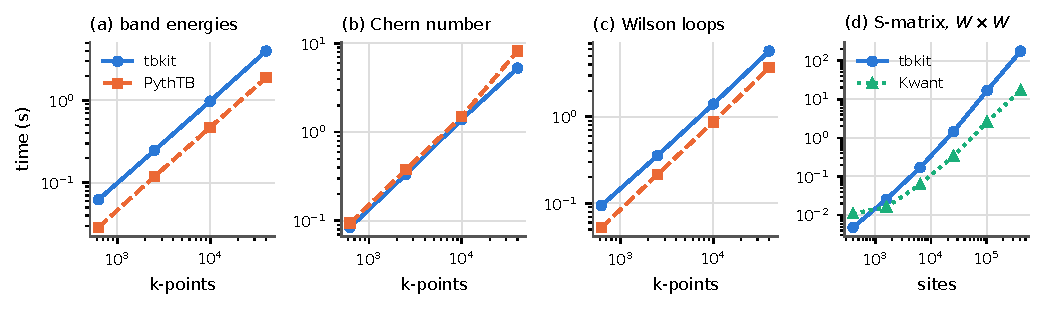
\includegraphics[width=\textwidth]{fig_benchmarks}
\caption{Wall-clock time on one thread. (a)--(c)~$k$-space tasks for a
random \benchnorb-orbital model on an $N\times N$ mesh, tbkit against PythTB.
(d)~Scattering matrix of a disordered $W\times W$ square device at one energy,
tbkit against Kwant (MUMPS). The two packages give the same transmission
to $10^{-8}$ at every size.}
\label{fig:benchmarks}
\end{figure}

We run each case in a fresh process with one BLAS thread, on an Apple M4
laptop (\benchplatform).
Peak memory is the growth of the resident set during the timed call
(Tables~\ref{tab:bench-kspace} and~\ref{tab:bench-transport}).

\begin{table}[t]
\centering\small
\caption{$k$-space tasks, \benchnorb{} orbitals, $\benchnk\times\benchnk$ mesh, one thread.}
\label{tab:bench-kspace}
\begin{tabular}{lrrrr}
\toprule
& \multicolumn{2}{c}{tbkit} & \multicolumn{2}{c}{PythTB} \\
Task & time (s) & memory (MB) & time (s) & memory (MB) \\
\midrule
\rows{tables/bench_kspace}
\bottomrule
\end{tabular}
\end{table}

\begin{table}[t]
\centering\small
\caption{Scattering matrix of a $W\times W$ device at one energy, one thread.}
\label{tab:bench-transport}
\begin{tabular}{rrrrr}
\toprule
& \multicolumn{2}{c}{tbkit} & \multicolumn{2}{c}{Kwant} \\
Sites & time (s) & memory (MB) & time (s) & memory (MB) \\
\midrule
\rows{tables/bench_transport}
\bottomrule
\end{tabular}
\end{table}

On Bloch meshes, tbkit and PythTB~2 scale alike [Fig.~\ref{fig:benchmarks}(a)--(c)].
Both are vectorized over $k$, and their run times stay within a factor of
about two. PythTB is faster for band energies and Wilson loops, and tbkit
is faster for the Chern number. tbkit's chunked eigensolver bounds its
memory, which is 5 to 14 times lower on the largest meshes. It can also use threads
(\code{KSpace.set\_workers}), which this single-thread comparison leaves
out. For transport, Kwant's MUMPS solver beats tbkit's SuperLU
factorization from about a thousand sites on, and the gap widens with size
[Fig.~\ref{fig:benchmarks}(d)]. At about $4\times10^5$ sites, Kwant is ten
times faster and uses less than a quarter of the memory. For large devices,
Kwant is the right tool. tbkit's transport is aimed at the models that a
user already builds for its band and topology tools, and at devices of up
to about $10^5$ sites, where it takes under 20 seconds on one thread.

%----------------------------------------------------------------------------
\section{Teaching}
\label{sec:teaching}

tbkit was written to be read as well as used. The gallery spans 20 topics,
from lattices to Floquet and non-Hermitian physics, and each example is a short
script that explains its physics and checks it. A history page of the
documentation tells the story of tight-binding physics as a chronology of
breakthroughs, from Bloch and Slater--Koster to moir\'e flat bands. Each
breakthrough links to examples that reproduce it, 73 links in all. The
two pipelines expose their intermediate objects (site arrays, bond tables,
sparse Hamiltonians), so a student can see how a model is assembled.

%----------------------------------------------------------------------------
\section{Availability and outlook}
\label{sec:outlook}

tbkit is distributed on PyPI (\code{pip install tbkit}) under the BSD
3-clause license. It requires NumPy, SciPy and matplotlib (SymPy for
$k\cdot p$ discretization). Its source, documentation and coverage report
are at \url{https://github.com/cpoli/tbkit} and
\url{https://cpoli.github.io/tbkit}. Every script behind this paper, from
validation and benchmarks to figures and listings, is in the \code{paper/}
directory of the repository.

The roadmap of the project lists the next steps. These include extending
lead interfaces automatically, moving the remaining Green's-function
transport onto the sparse factorization, energy-parallel transport, import
and export of Kwant and PythTB models, and Hartree--Fock on Bloch meshes.

\section*{Acknowledgements}
% TODO: acknowledgements and funding.

\bibliographystyle{unsrt}
\bibliography{references}

\end{document}
